\chapter{Overzicht}

\par De toplaag combineert alle onderliggende lagen om een functioneel geheel te verkrijgen.
Als inputs heeft de toplaag enkel objecten waarop de gebruiker effectief kan interageren zoals knoppen of een audio aansluiting.
Ook de outputs zijn direct merkbaar door de gebruiker, zijnde een HDMI of OLED scherm, of LEDs om de status aan te duiden.

\section{Input}

	\par Door middel van 6 schakelaars en een audio interface is de gebruiker in staat om de inputs zelf aan te passen. Door gebruik van de schakelaars kan de voorstellingswijze van het spectrum op het HDMI scherm gekozen worden. Via een resetknop kunnen de verschillende componenten terug ingesteld worden op hun initi\"ele waarde. 

	\par Doordat er gewerkt wordt met een externe geluidsbron is het mogelijk om eender welke audio af te spelen via de 3.5mm audio jack. Hierin voert men een signaal toe dat afkomstig kan zijn van een PC of mp3-speler, 

\section{Output}

	\par Op het OLED scherm dat aanwezig is op het ZedBoard wordt weergegeven wat de huidige instellingen zijn. Deze instellingen worden aangepast door middel van de schakelaars. Tijdens de opstartfase wordt een vaste text weergegeven gedurende 4 seconden. Hierna wordt overgegaan naar de modus met die de instellingen weergeeft.

	\par Via de HDMI uigang wordt het frequentiespectrum weergegeven op een HDMI-compatibel scherm. 

	\par De binnengelezen audio zal ook weer naar buitengebracht worden zodat de gebruiker via de koptelefoon in staat is de audio te beluisteren die bij het weergegeven frequentiespectrum hoort. 

	\par Wanneer een schakelaar van postie veranderd zal ook het bijhorend ledlampje oplichten. Hierbij is ook rekening gehouden met de onderlinge afhankelijkheid tussen verschillende modi. 


\section{Mapping}
	
	\begin{figure}[H]
		\centering
		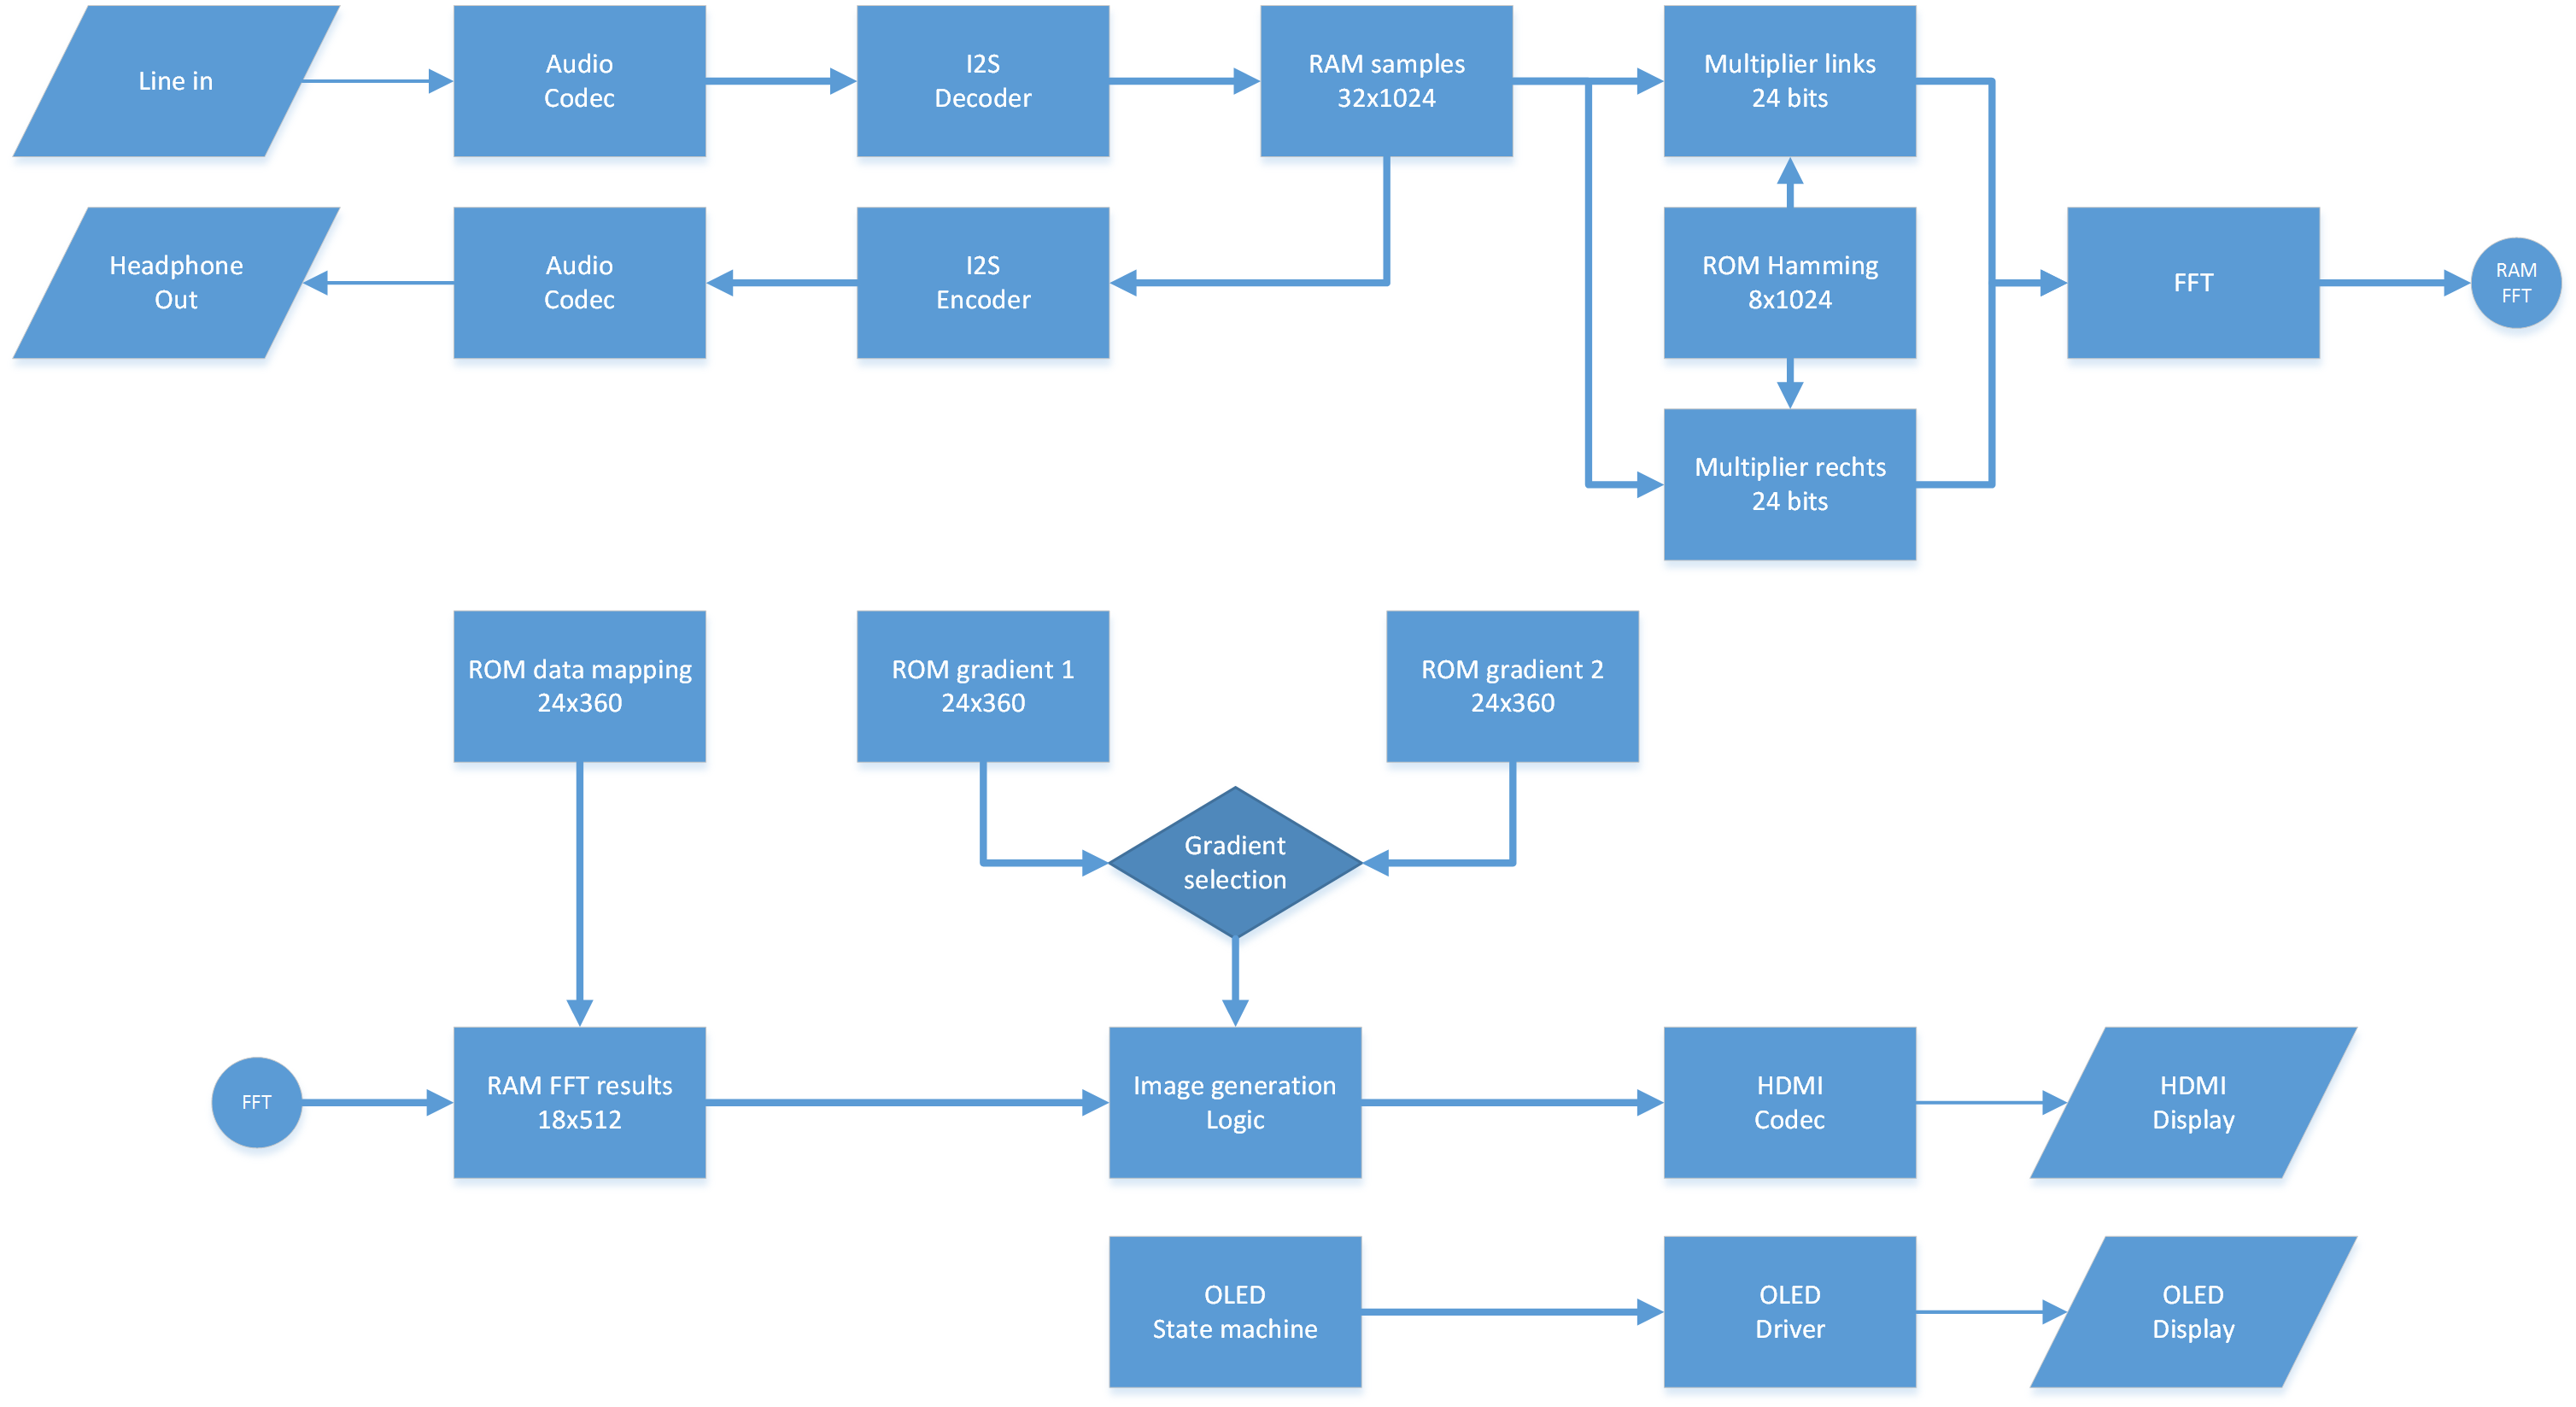
\includegraphics[width=0.8\textwidth]{Chapters/GlobaalSchema/Images/Global.png}
		\caption{Globaal overzicht van de audio equalizer}
		\label{fig:globaal_overzicht}
	\end{figure}

	\par In figuur \ref{fig:globaal_overzicht} is een globaal overzicht weergegeven van de verschillende componenten en hoe deze verbonden zijn met elkaar. Een grotere versie van deze figuur is toegevoegd in appendix \ref{sec:appMapping} op bladzijde \pageref{sec:appMapping}.

		\begin{enumerate}
			\item Een audiosignaal wordt aangelegd aan de lijningang van het ZedBoard.
			\item Het audiosignaal wordt binnengelezen door middel van de audiocodec ADAU1761.
			\item Het audiosignaal wordt gedecodeerd door middel van een I\textsuperscript{2}S decoder
			\item Een RAM geheugen wordt gevuld tot er 1024 audiosamples in aanwezig zijn. Elk sample bestaat uit 16-bit audiodata per kanaal.
			\item Wanneer het audiosample geheugen volledig gevuld is worden de samples een voor een uitgelezen en vermenigvuldgt met een hamming window waarde. Dit gebeurt afzonderlijk voor elk kanaal. 
			\item De audiosamples worden vervolgens aangevoerd aan de FFT component. Deze leest ook 1024 samples in alvorens de transformatie begint.
			\item Wanneer de transformatie klaar is worden de samples opgeslagen in een RAM geheugen. De 512 samples worden geschaald naar een breedte van 1280 pixels. 
			\item Tot slot zal de Image generation logic afhankelijk van de schakelaars een beeld genereren dat op het scherm wordt weergegeven. 
		\end{enumerate}

		\par Wanneer de gebruiker een schakelaar van positie wijzigt zal op het OLED scherm een passende tekst worden weergegeven die aantoont welke modus er actief is.


\section{Process}

	\par Bij de opstart van het ZedBoard zal een state-machine doorlopen worden. In een eerste fase zal het OLED scherm worden ge\"initialiseerd. In een tweede fase zal gedurende 4 seconden een vaste tekst op het OLED scherm weergegeven worden. Vervolgens wordt overgegaan naar een derde fase waar een andere tekst ook 4 seconden wordt weergegeven. Wanneer deze 8 seconden voorbij zijn wordt er gereageerd op de gebruikersinvoer. Het OLED scherm zal vanaf dan de actuale status weergeven van de schakelaars. Op het HDMI scherm wordt continu het spectrum van de binnenkomende audio weergegeven.

	\par Het process in het top level voorziet ook in de vertraging van verschillende signalen die worden doorgegeven aan de verschillende systeemcomponenten zodat de data steeds op het juiste moment bij de component toekomt. Een overzicht van de hiervoor gevolgde statemachine is terug te vinden in bijlage \ref{sec:appTop}.

\section{Gebruikte IPs}

	\begin{description}
		\item[clk\_wiz\_0:] (Clocking Wizard) Deze IP staat in voor het genereren van de klokken die nodig zijn binnen het project. Er wordt een klok van 100 MHz en 12.288 MHz gegenereerd. 
		
		\item[audio\_sample\_block\_mem:] (Block Memory Generator) In dit RAM geheugen worden de audiosamples opgeslagen die binnengelezen worden door middel van de audiocodec. Door middel van een adresgenerator worden de in- en uitleesadressen voor dit geheugen gegenereerd. De invoer van data is rechtstreeks afkomstig van de audiocodec. De uitvoer gaat via de hamming window multiplier naar de FFT.  
		
		\item[block\_mem\_hamming:] (Block Memory Generator) Dit ROM geheugen zijn de waarden voor het hamming window opgeslagen. Het adres dat gebruikt wordt om het audio sample geheugen uit te lezen zal 2 kloktikken vertraagd worden zodat het ook kan gebruikt worden om het adres van dit geheugen te genereren. De uitvoer van dit geheugen (de hamming window waarde voor het overeenkomstig samplenummer) zal worden aangelegd aan de hamming window multiplier.
		
		\item[hamming\_multiplier\_left:] (Multiplier) Deze component zorgt voor het vermenigvuldigen van het linker kanaals audiosample met de waarde van het hamming window. Vervolgens wordt de data aangevoerd aan de FFT.
		
		\item[hamming\_multiplier\_right:] (Multiplier) Deze component zorgt voor het vermenigvuldigen van het rechter kanaals audiosample met de waarde van het hamming window. Vervolgens wordt de data aangevoerd aan de FFT.
		
		\item[FFT\_LR:] (FFT) Deze component voert de FFT transformatie uit op 1024 samples. Deze samples zijn afkomstig uit het audio sample geheugen, maar zijn eerst vermenigvuldigd met een hamming window. Wanneer aangegeven wordt dat het laatste sample is binnen gelezen start de FFT component met het berekenen van het spectrum. Wanneer deze klaar is wordt een FIN-vlag op hoog gezet. Vervolgens wordt deze data opgeslagen in het FFT output geheugen.
		
		\item[FFT\_output\_mem:] (Block Memory Generator)  In dit geheugen wordt de uitvoer van de FFT opgeslagen. Wanneer de HDMI VGA nieuwe data nodig heeft leest deze dit geheugen uit. Vervolgens kan op het scherm het spectrum weergegeven worden.
	\end{description}

\section{ZedBoard Pinout}
	
	\begin{figure}[H]
		\centering
		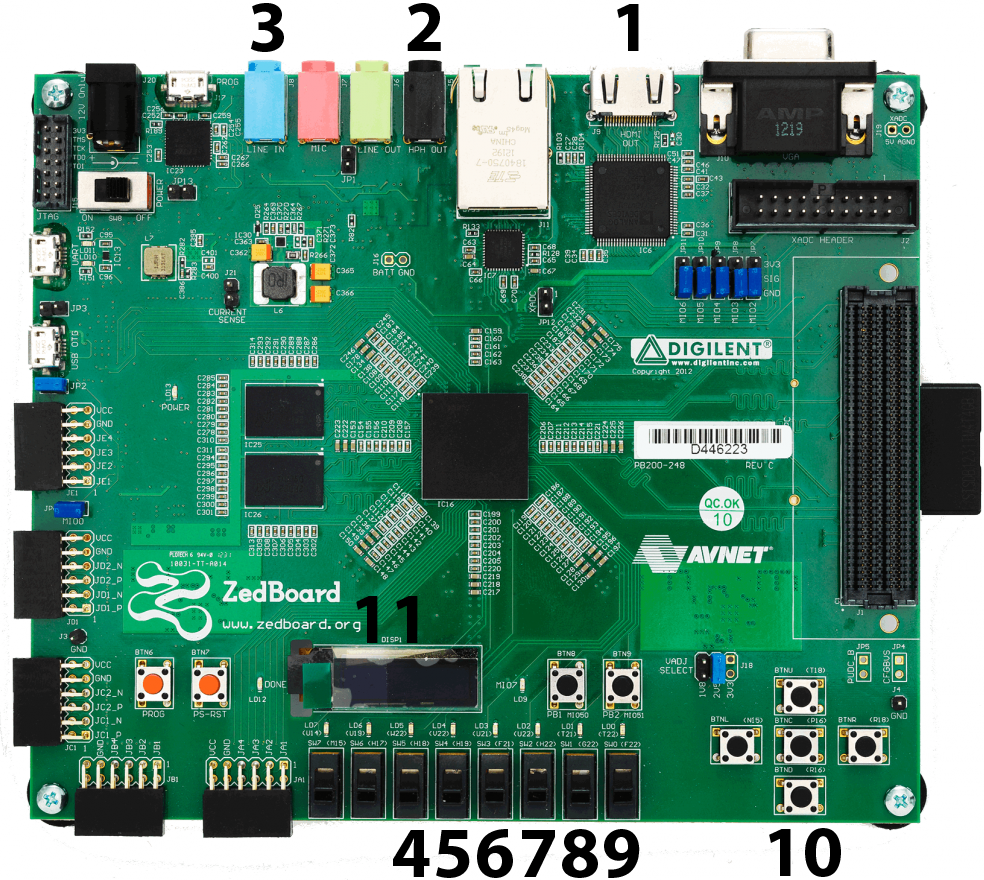
\includegraphics[width=0.9\textwidth]{Chapters/GlobaalSchema/Images/zedboard_large_transparent_nr.png}
		\caption{Weergave van de gebruikte componenten op het ZedBoard}
		\label{fig:zedboard_gebruikte_componenten}
	\end{figure}

\newpage
	\begin{description}
		\item [HDMI uitvoer:] Via deze aansluiting kan een HDMI scherm aangesloten worden waarop het audiospectrum zal worden weergegeven. \lbrack 1\rbrack 
		
		\item [Audiouitvoer naar hoofdtelefoon:] De audio kan beluisterd worden door middel veen een hoofdtelefoon die aangesloten wordt op de hph out connectie. \lbrack 2\rbrack
		
		\item [Audioinvoer:] Audio wordt aangevoerd via de line-in plug op het ZedBoard. \lbrack 3\rbrack
		
		\item [Schuifknop voor rounded rectangle mode:] Hiermee kan men de blokjes uit het discreet spectrum een lichte afronding geven, een aangenaam visueel effect. \lbrack 4\rbrack
		
		\item [Schuifknop voor averaging aan/uit:] Met deze schakelaar kan de uitmiddeling in of uitgeschakeld worden. Dit zorgt voor een vloeiender verloop van het spectrum. \lbrack 5\rbrack
		
		\item [Schuifknop voor rectangles aan/uit:] Hiermee kan er gewisseld worden tussen een nagenoeg continu spectrum en amplitude en een discreet spectrum en amplitude.\lbrack 6\rbrack
		
		\item [Schuifknop voor thema selectie jet/orange:] Hiermee kan gekozen worden tussen 2 gradi\"enten. De zogenaamde jet kleuren en een oranje thema.\lbrack 7\rbrack
		
		\item [Schuifknop voor edgemode:] Met deze schakelaar kan gekozen worden om enkel de buiteste rand van het spectrum volledig te kleuren. De rest wordt dan half zo helder afgebeeld.\lbrack 8\rbrack
		
		\item [Schuifknop voor peakmode:] Hiermee kan gekozen worden om het spectrum af te beelden als een punt in plaats van als balk. Dan wordt enkel het bovenste deel van de balk afgebeeld, de rest is de achtergrondkleur.\lbrack 9\rbrack
		
		\item [Resetknop:] Deze knop zorgt voor een resetactie in het toplevel. Indien een bepaalde component ook een reset ingang heeft dan wordt deze knop ook met deze ingang verbonden.\lbrack 10\rbrack
		
		\item [OLED scherm:] Data over de actieve modus wordt weergegeven op het OLED scherm. Wanneer een modus wijzigt zal ook de tekst worden aangepast. \lbrack 11\rbrack
	\end{description}	

